\chapter{$b$-tagging performance at high $p_{T}$}
\label{AppendixB}

One of the limiting factors of the signal acceptance in the $FourBfull$ search at high resonance masses is the degradation of the $b$-tagging efficiency for high $p_{T}$ jets. This appendix presents a study of the underlying causes of this degradation. 

\section{MV2 algorithm overview}

The MV2 algorithm is a boosted decision tree incorporating twenty-four input variables constructed from three lower level input algorithms: IPxD, SV1, and JetFitter. IPxD uses the two and three dimensional impact parameter information of tracks in the jet to construct templates for light, charm, and bottom quarks and compute likelihood ratios. SV1 is a secondary vertex reconstruction algorithm. JetFitter atemtps to fit to the full decay chain of the $B$ hadron, looking for multiple decay vertices aligned along a single axis. Figure~\ref{fig:MV2inputs} summarizes the inputs to MV2. 

\begin{figure}[h!]
  %\vspace{20pt}
  \centering
  \captionsetup{justification=centering}

  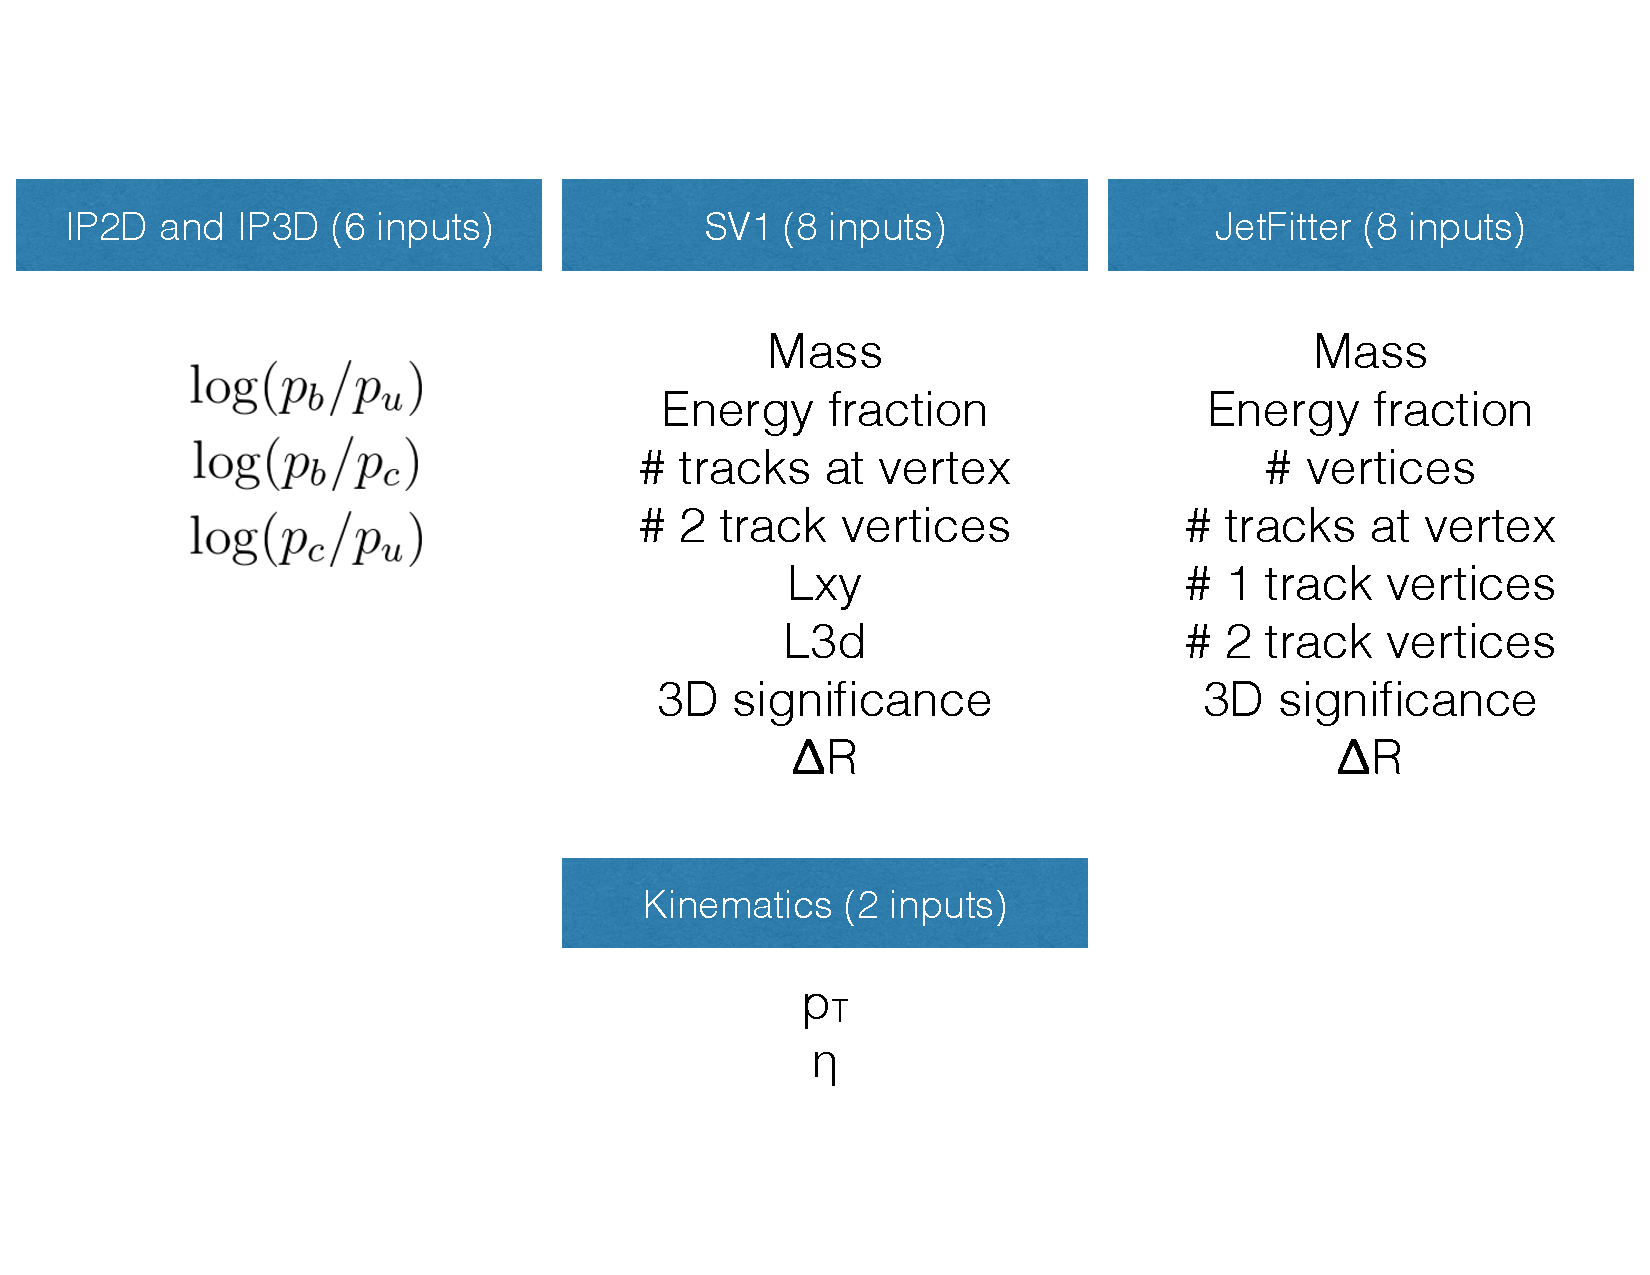
\includegraphics[width=0.7\textwidth]{figures/MV2_inputs}
  \caption{Summary of the inputs to the MV2 $b$-tagging algorithm}
  \label{fig:MV2inputs}
\end{figure}

\section{Changes in MV2 score at high $\pT$}

The degradation of $b$-tagging at high $\pT$ was studied in particular in the context of RSG models at high mass. Figure~\ref{fig:TrackJetPt} shows the $\pT$ of the leading track jet inside of the leading calorimeter jet in RSG events. At high $m_{\Gkk}$, the $\pT$ spectrum of track jets is much harder than at lower masses due to the increased Higgs $\pT$. 

\begin{figure}[h!]
  %\vspace{20pt}
  \centering
  \captionsetup{justification=centering}

  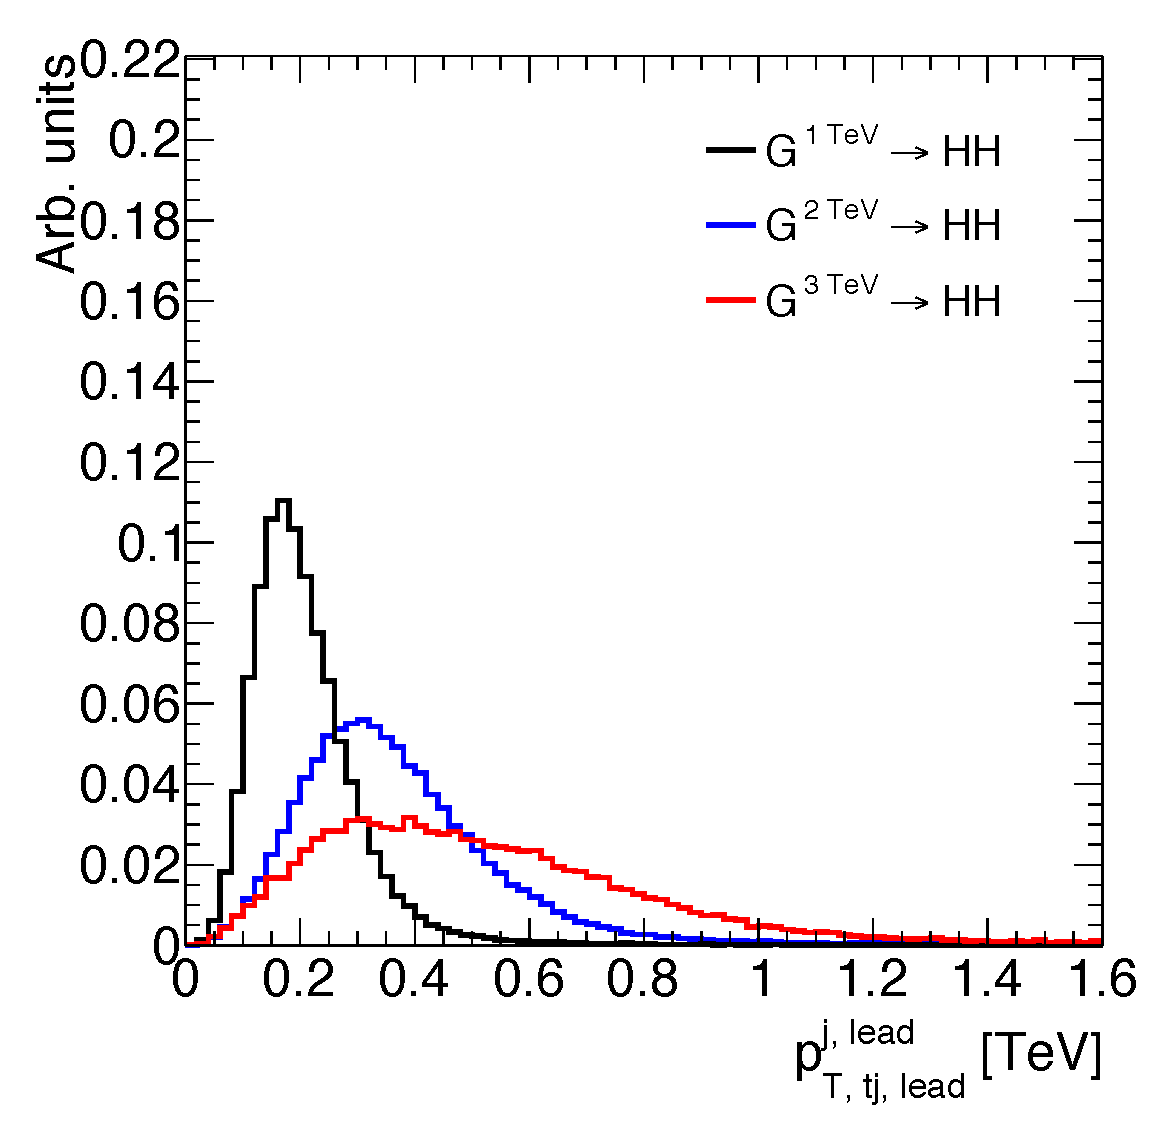
\includegraphics[width=0.5\textwidth]{figures/TrackJetPt}
  \caption{$\pT$ of the leading track jet in the leading calorimeter jet for different signal masses in RSG $c=1$ models}
  \label{fig:TrackJetPt}
\end{figure}

Figure~\ref{fig:TrackJetMV2} shows the MV2c20 algorithm score for the leading and subleading track jets inside of the leading calorimeter jet. In both cases, it can be seen that at higher RSG masses the MV2 score shifts towards more background like (negative) values. Additionally, this effect is more pronounced in the leading track jet than the subleading. 

\begin{figure}[h!]
  %\vspace{20pt}
  \centering
  \captionsetup{justification=centering}

   \begin{subfigure}[t]{0.5\textwidth}
        \centering
        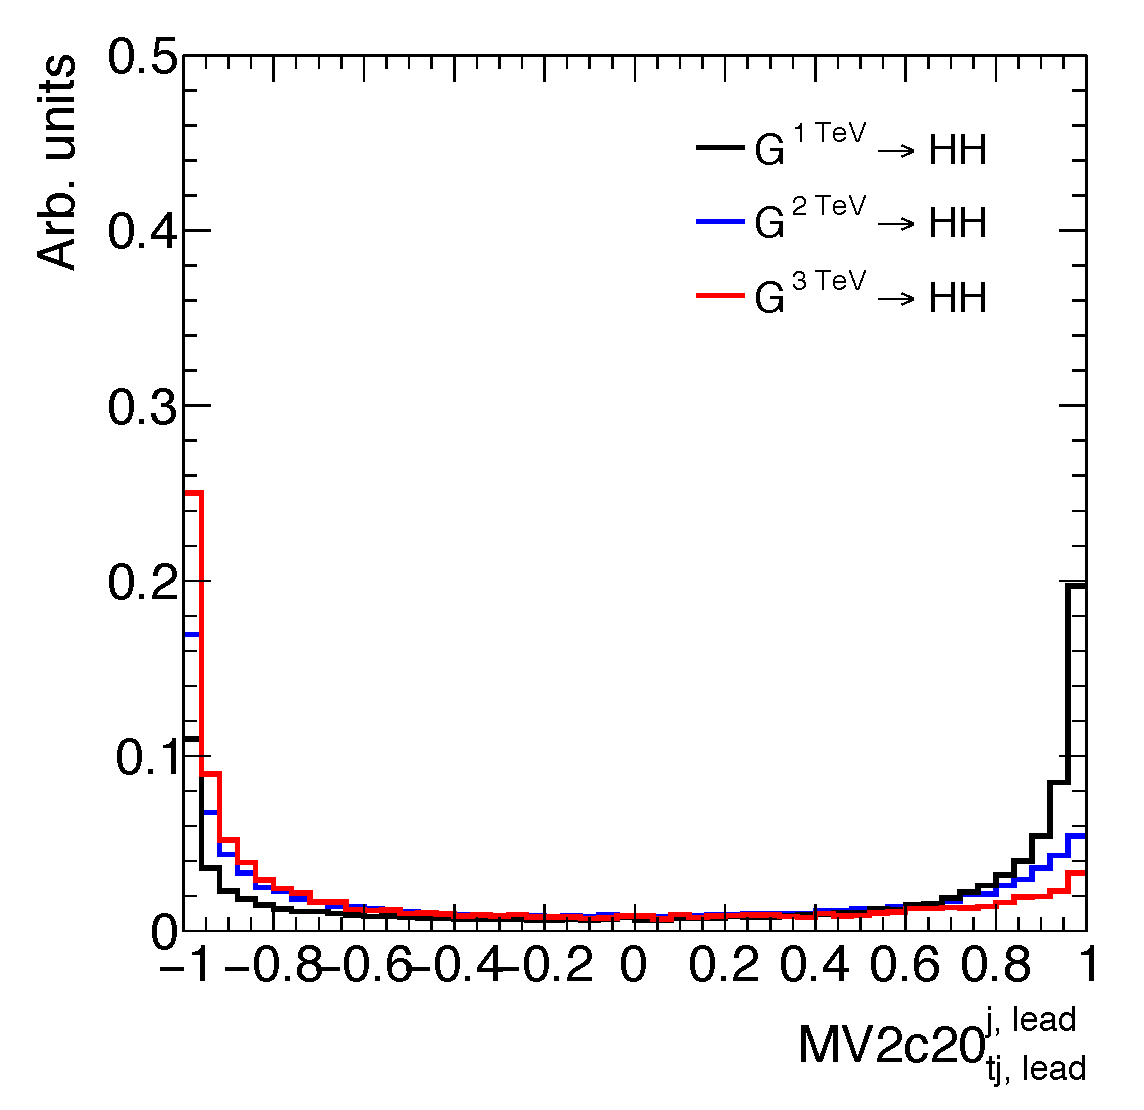
\includegraphics[width=\textwidth]{figures/LeadTrackJet_MV2c20}
        \caption{}
    \end{subfigure}%
    \begin{subfigure}[t]{0.5\textwidth}
        \centering
        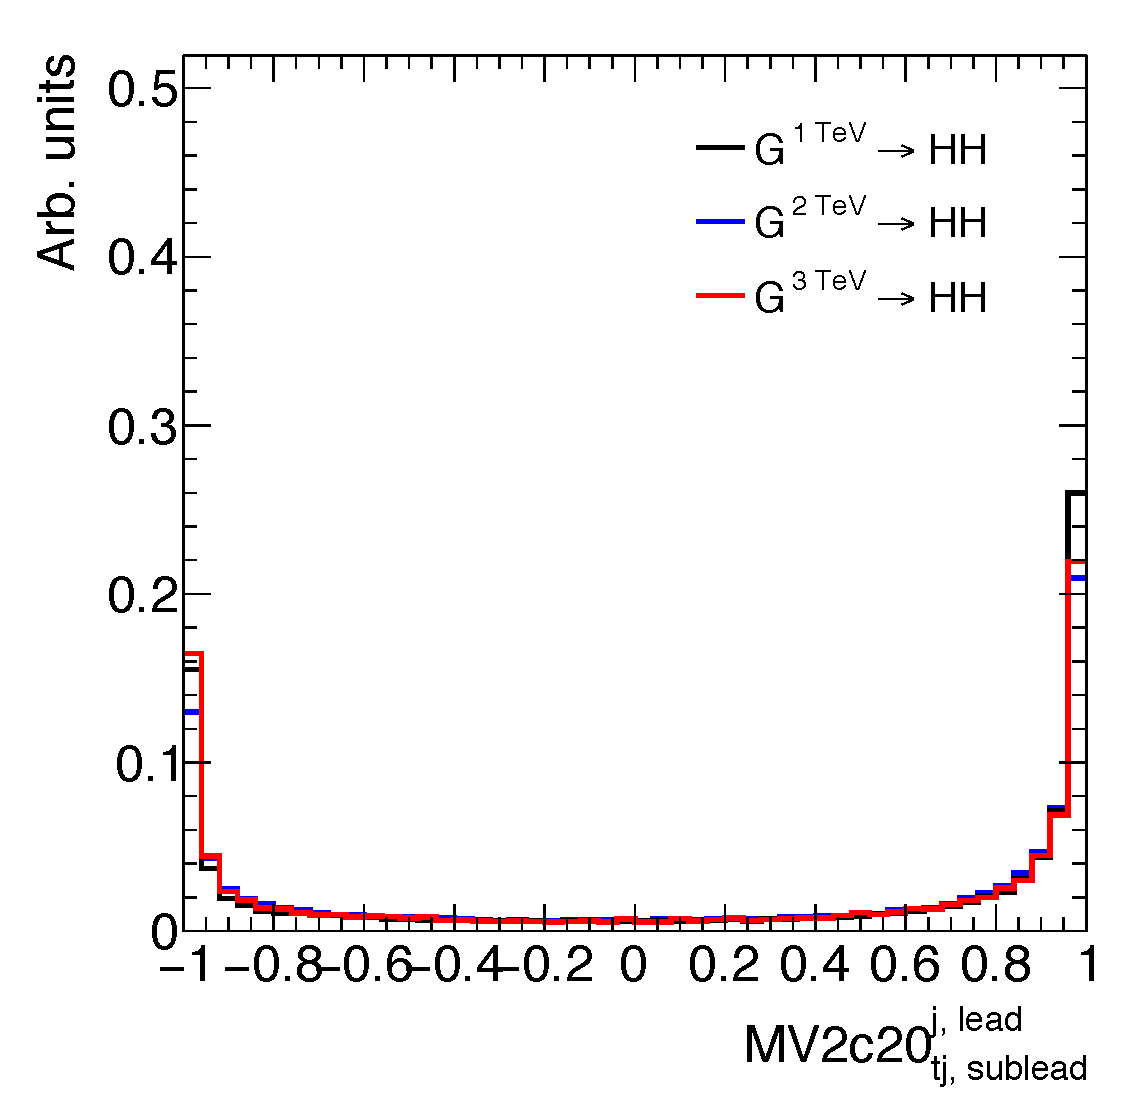
\includegraphics[width=\textwidth]{figures/SubleadTrackJet_MV2c20}
        \caption{}
    \end{subfigure}

   \caption{MV2c20 score for the leading track jet (a) and subleading track jet (b) of the leading calorimeter jet for different signal masses in RSG $c=1$ models}
  \label{fig:TrackJetMV2}
\end{figure}

To understand what is causing this change in the MV2c20 score, the same comparisons can be made for the input variables of MV2c20. The focus in these comparisons will be on the leading track jet as this is the one seen to have the largest difference in MV2 score. Figure~\ref{fig:TrackJetIP3D} shows the log likelihood ratio $\log(p_b/p_u)$ from the IP3D (three dimensional impact parameter) algorithm. At higher masses, the IP3D likelihood ratio distribution does become more background-like. 

\begin{figure}[h!]
  %\vspace{20pt}
  \centering
  \captionsetup{justification=centering}

  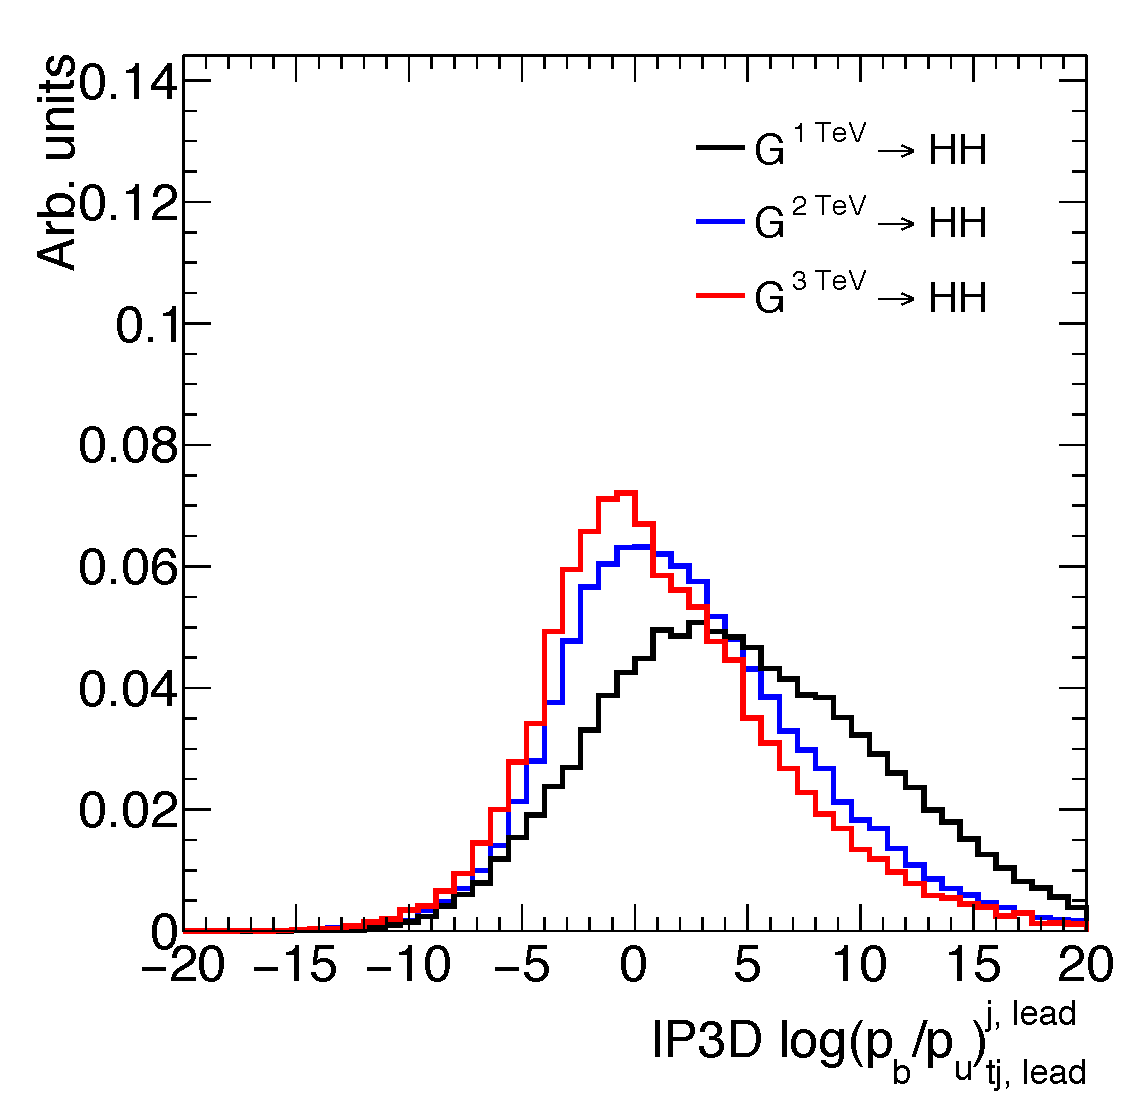
\includegraphics[width=0.5\textwidth]{figures/LeadTrackJet_IP3D}
  \caption{IP3D log-likehood ratio ($\log(p_b/p_u))$) of the leading track jet in the leading calorimeter jet for different signal masses in RSG $c=1$ models}
  \label{fig:TrackJetIP3D}
\end{figure}
%
Figure~\ref{fig:TrackJetSV1} shows the mass and number of tracks at the secondary vertex computed by the SV1 algorithm. When there is no secondary vertex found, the algorithm assigns a default negative value for these quantities. Both of these distributions show that there is a significantly larger fraction of jets where no secondary vertex is found in the high mass samples compared to the $m_{\Gkk} = 1 \TeV$ sample. The SV1 algorithm's inability to find a secondary vertex could be an important factor in the overall MV2 score shift, as this eliminates eight of the input variables that would normally contribute information to the algorithm. 

\begin{figure}[h!]
  %\vspace{20pt}
  \centering
  \captionsetup{justification=centering}

   \begin{subfigure}[t]{0.5\textwidth}
        \centering
        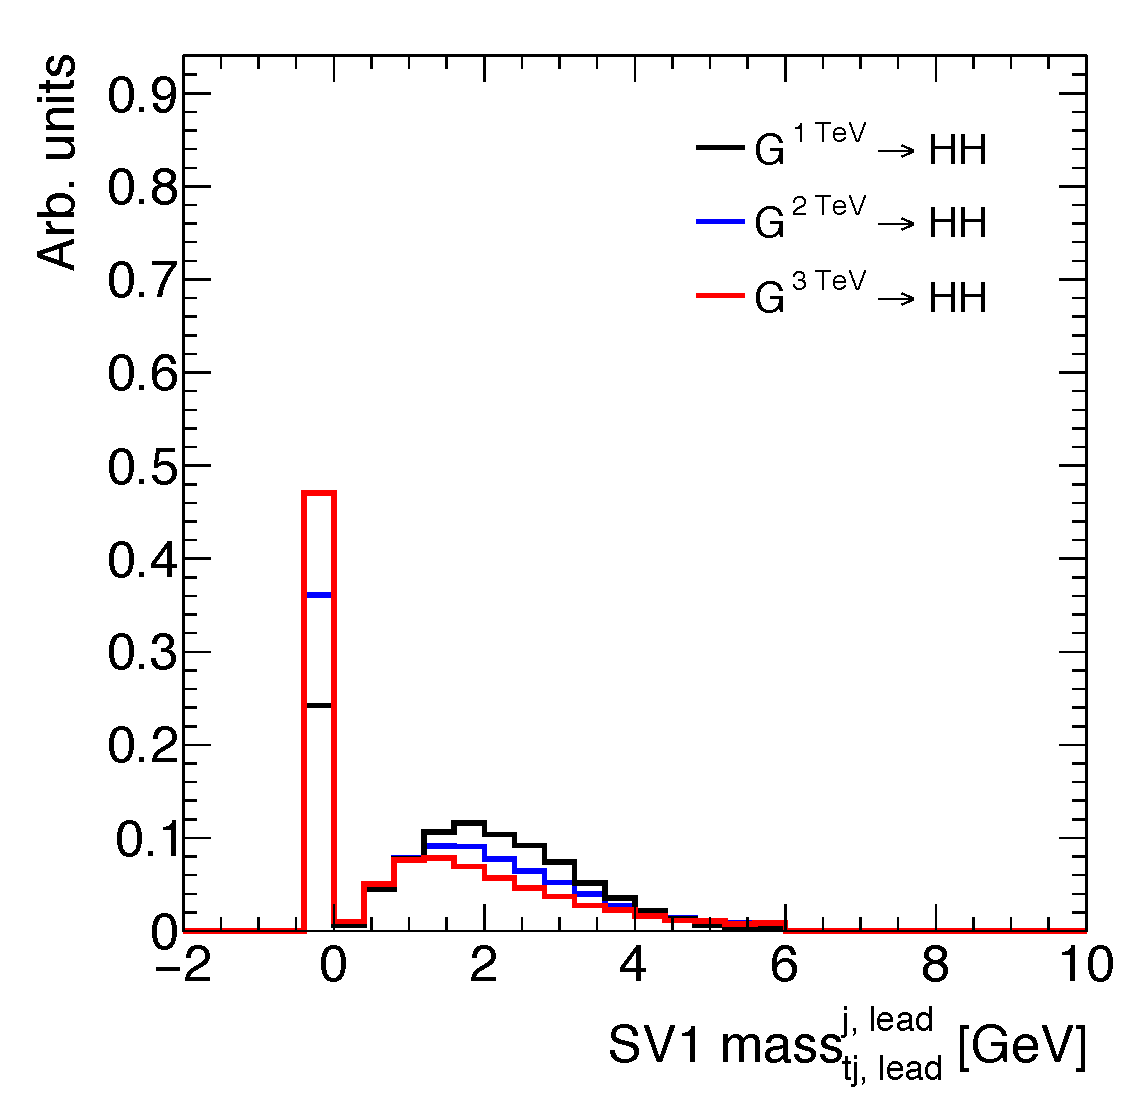
\includegraphics[width=\textwidth]{figures/LeadTrackJet_SV1mass}
        \caption{}
    \end{subfigure}%
    \begin{subfigure}[t]{0.5\textwidth}
        \centering
        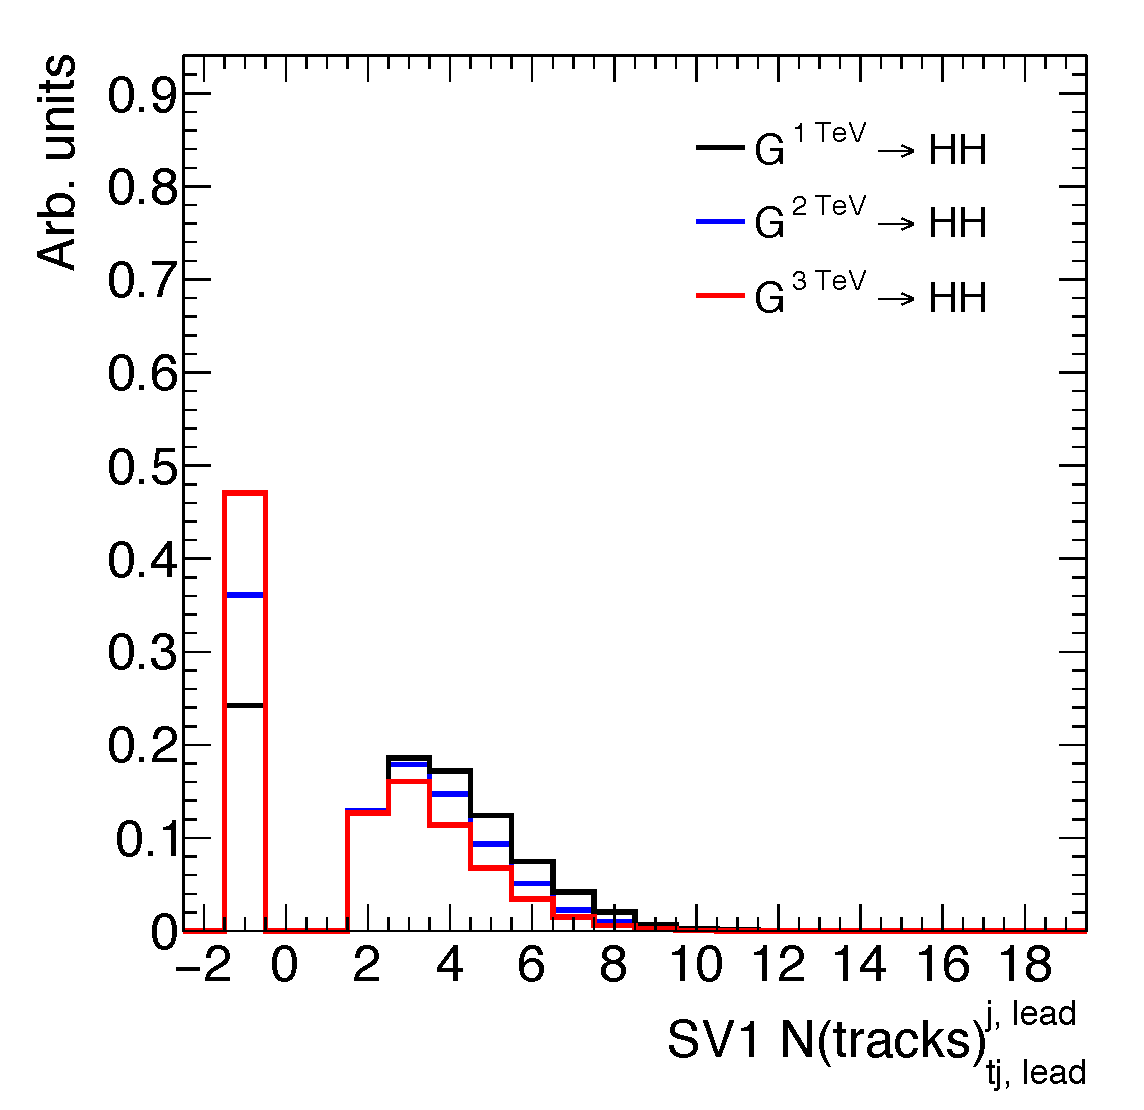
\includegraphics[width=\textwidth]{figures/LeadTrackJet_SV1ntrk}
        \caption{}
    \end{subfigure}

   \caption{Mass (a) and number of tracks (b) for the secondary vertices computed with the SV1 algorithm. When no secondary vertex is found, the quantiites are assigned to default negative values.}
  \label{fig:TrackJetSV1}
\end{figure}

Figure~\ref{fig:TrackJetJF} shows the same quantities for the JetFitter algorithm. In this case, there is also a change in the fraction of jets which have their secondary vertices successfully reconstructed, but this change is not as drastic as that seen in SV1. There is also an increase in the number of jets which have high values of mass. 

\begin{figure}[h!]
  %\vspace{20pt}
  \centering
  \captionsetup{justification=centering}

   \begin{subfigure}[t]{0.5\textwidth}
        \centering
        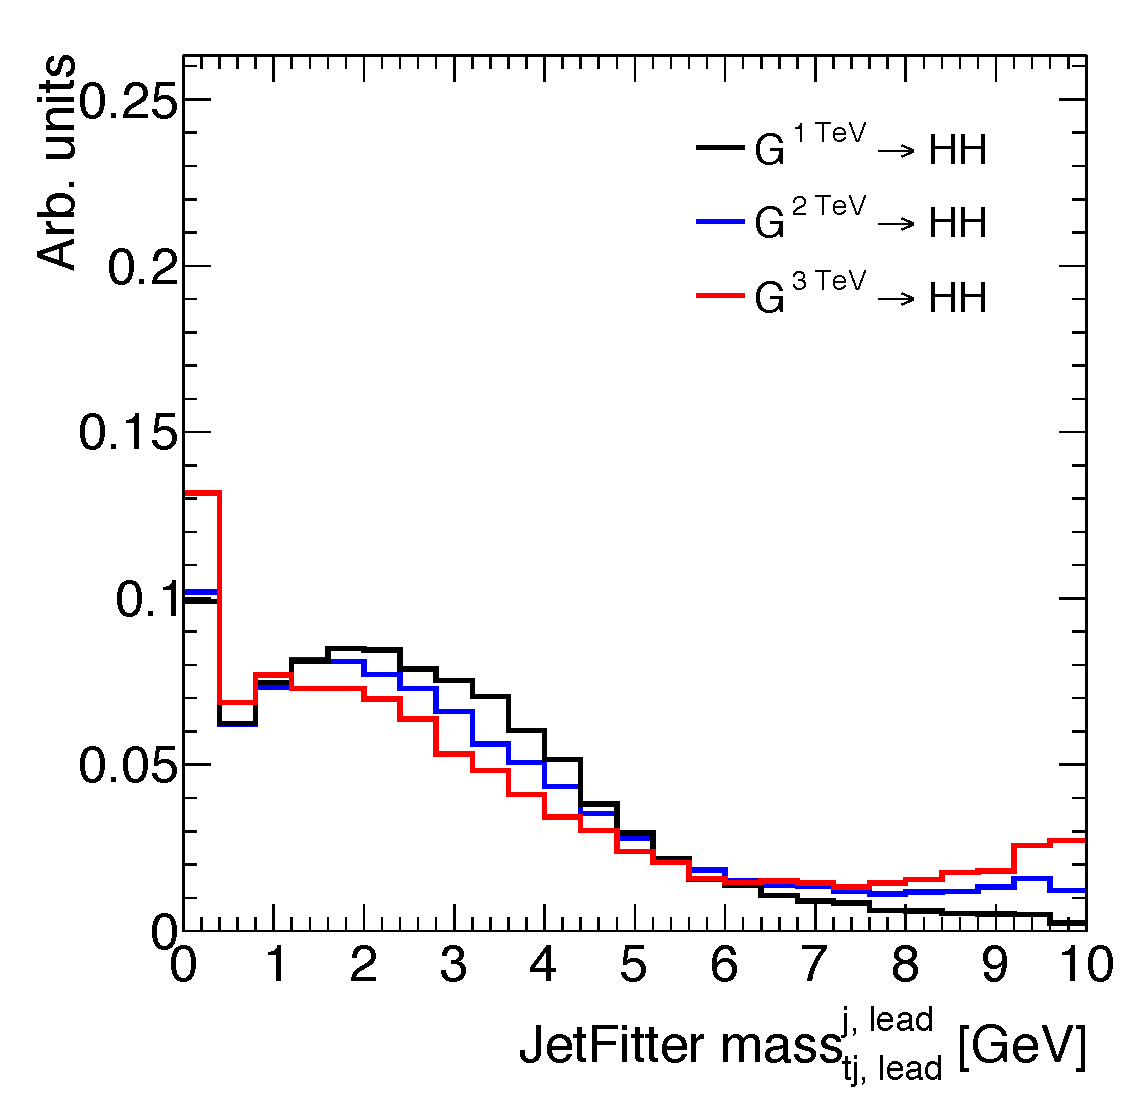
\includegraphics[width=\textwidth]{figures/LeadTrackJet_JFmass}
        \caption{}
    \end{subfigure}%
    \begin{subfigure}[t]{0.5\textwidth}
        \centering
        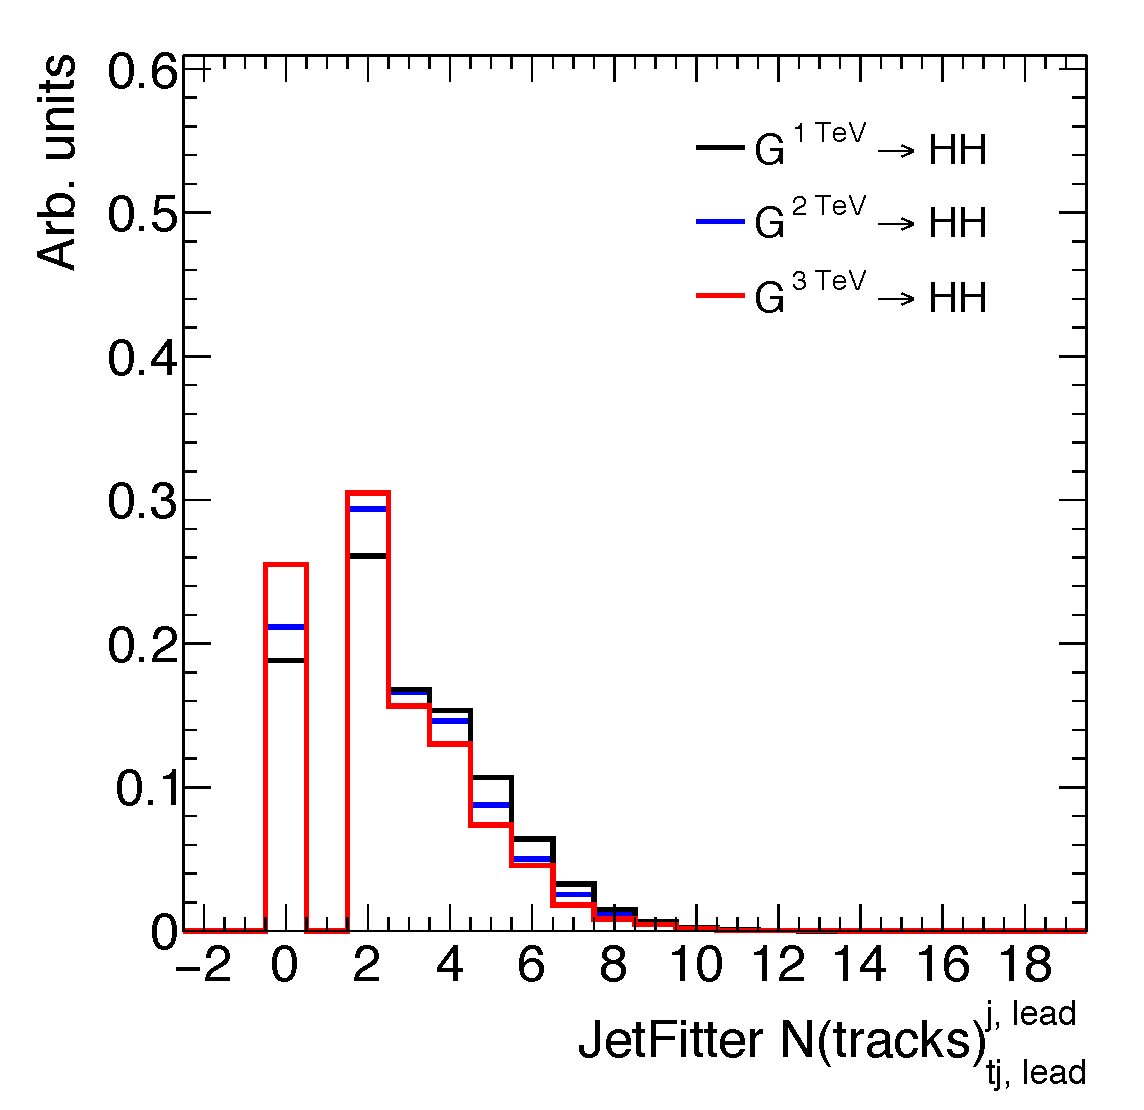
\includegraphics[width=\textwidth]{figures/LeadTrackJet_JFntrk}
        \caption{}
    \end{subfigure}

   \caption{Mass (a) and number of tracks (b) for vertices computed with the JetFitter algorithm. When no vertices are found, the quantiites are assigned to default negative values.}
  \label{fig:TrackJetJF}
\end{figure}

\section{Tagging efficiency by individual jet}

In the last section, the largest changes in MV2 score were seen for the leading track jet inside the leading calorimeter jet. To confirm that the overall $4b$ tagging efficiency is indeed degrading because of degradation of the leading track jet efficiency, the tagging efficiency for each individual jet as a function of mass can be compared. This is shown in figure~\ref{fig:btag_ind_jet}. The figure shows that the leading jet tagging efficiency in both calorimeter jets degrades heavily, while the sub-lead jet tagging efficiency remains relatively constant.

\begin{figure}[h!]
  %\vspace{20pt}
  \centering
  \captionsetup{justification=centering}

  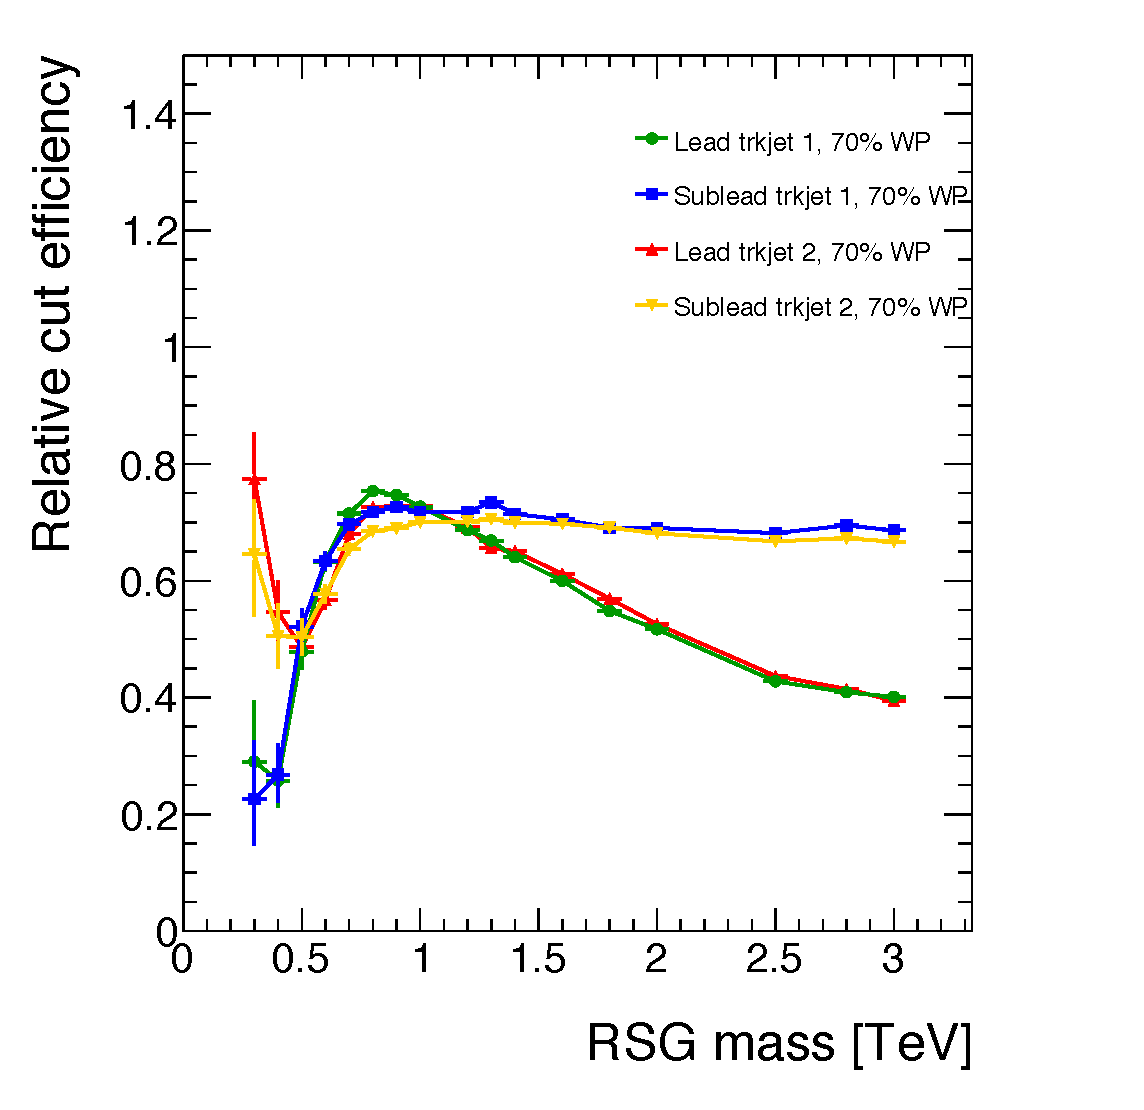
\includegraphics[width=0.5\textwidth]{figures/Btag_singlejet_comparison}
  \caption{MV2c20 $b$-tagging efficiency for each of the four track jets in the boosted $4b$ selection as a function of RSG mass for $c=1$ models.}
  \label{fig:btag_ind_jet}
\end{figure}

\section{Effect of multiple $b$-quarks inside one jet}

One hypothesis for why the efficiency of $b$-tagging the leading track jet degrades is that at high masses, the $b$ quarks get close enough together that both of them are inside of the leading track jet. Because MV2 is not tuned for tagging multiple $b$ quarks inside one jet, the tagging efficiency could degrade. Figure~\ref{fig:MV2_nb} shows MV2 scores and SV1 mass for cases where there are two $b$ quarks at truth level within the radius of the leading track jet compared to cases where there is only one true $b$\footnote{When two truth $b$ quarks are required in the leading jet, the subleading jet is required to have zero. When one is required for the leading, one is also required for the subleading.}. 

\begin{figure}[h!]
  %\vspace{20pt}
  \centering
  \captionsetup{justification=centering}

   \begin{subfigure}[t]{0.5\textwidth}
        \centering
        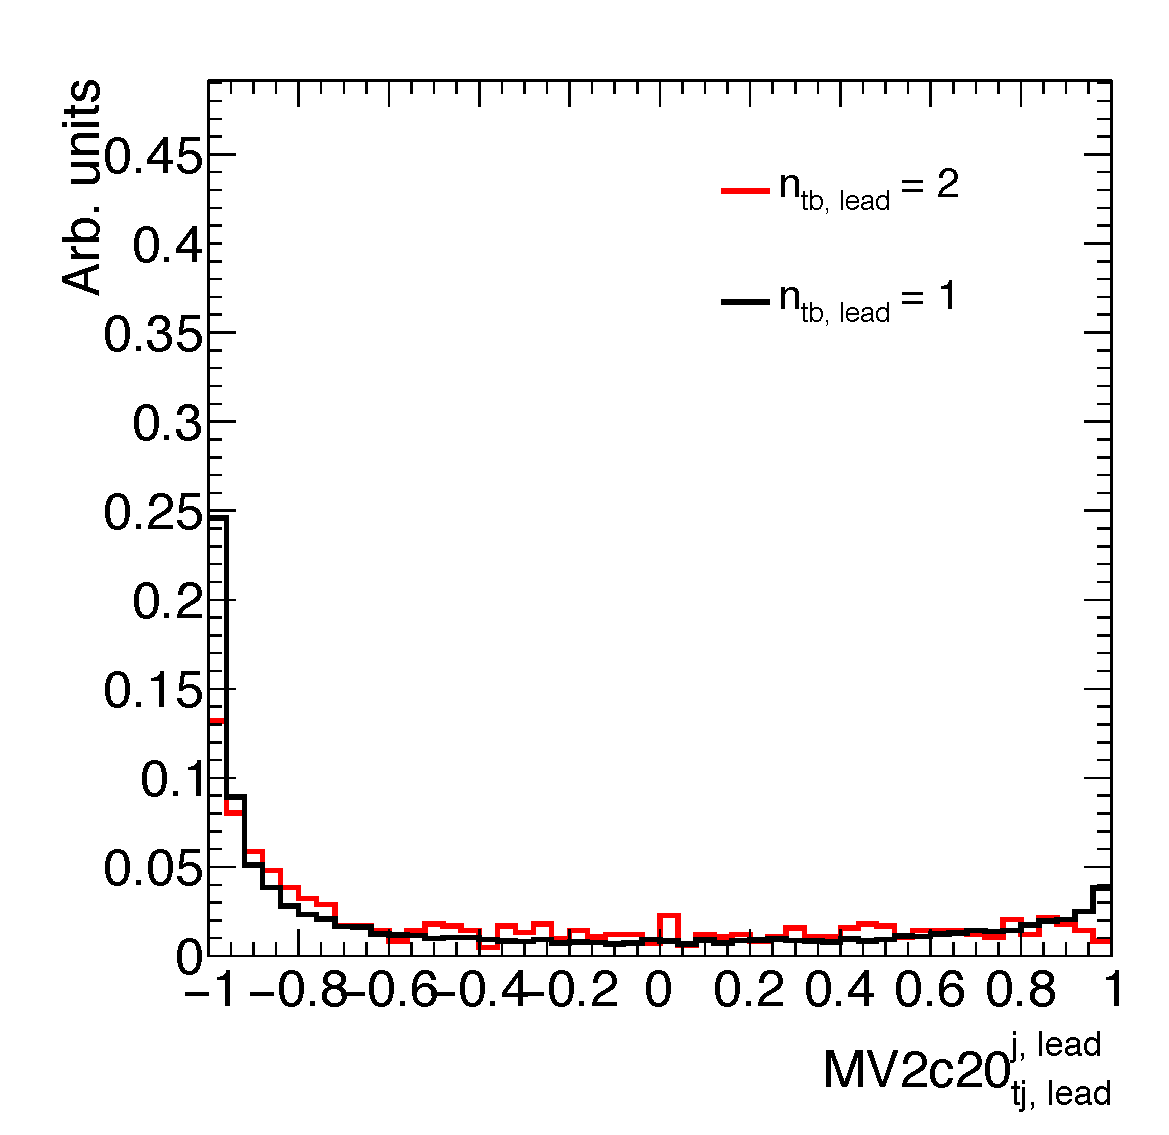
\includegraphics[width=\textwidth]{figures/Ntb_MV2c20}
        \caption{}
    \end{subfigure}%
    \begin{subfigure}[t]{0.5\textwidth}
        \centering
        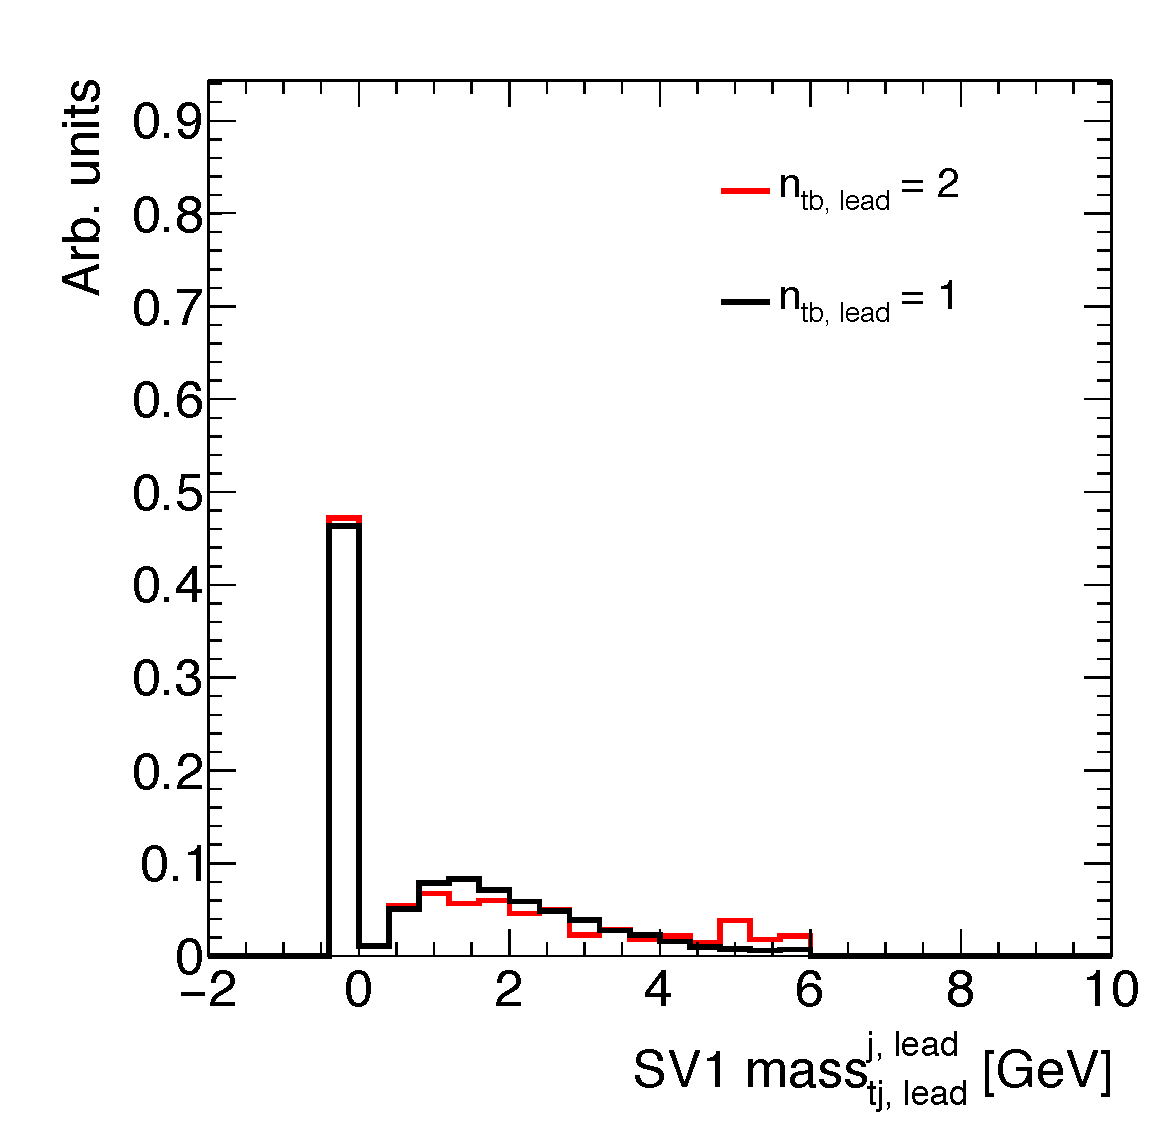
\includegraphics[width=\textwidth]{figures/Ntb_SV1mass}
        \caption{}
    \end{subfigure}

   \caption{MV2c20 score (a) and SV1 mass (b) for leading track jets with two truth $b$ quarks ($n_{\rm tb, lead} = 2$) compared to those with only one truth $b$ ($n_{\rm tb, lead} = 1$).}
  \label{fig:MV2_nb}
\end{figure}

\section{Changes in track quality at high $\pT$}

To investigate the change in MV2 score further, individual track quantities within the jet can be compared. 





